% Session 8 -- valence bond solid versus resonating valence bond: a fixed dimer covering
% Placement: end of sec. "The QSL ground state: the resonating valence bond wavefunction",
% referenced from the dimerized-Heisenberg section as well.
% Rendered by figures/blender/s08f03_vbs_rvb.py, labels in figures/overlays/s08f03_vbs_rvb.tex.
\begin{aqmfigure}{fig:s08:vbsrvb}{The difference between a valence bond solid and a quantum spin
liquid is not whether the ground state is built from singlets, since both are, but whether the
singlet pattern is frozen. (a1) The fully dimerized model (8.4) has one fixed covering, (8.5). (a2)
When we separate the two unpaired spins of figure~\ref{fig:s08:magnonspinon}b, every strong bond
between them loses its singlet, drawn in red, so the energy cost grows with the separation. The pair
is confined, and only the bound object propagates, which is the spin-$1$ triplon. (b1) The RVB state
(8.7) is a superposition over \emph{all} pairings, near and far, drawn as coverings stacked on top
of each other. (b2) Now the background pairs again behind the excitations with no cost, the
confining string does not form, and the two halves separate as independent spin-$1/2$ spinons.
Frustration is the reason why the superposition in (b1), and not a single covering, is the ground
state.}
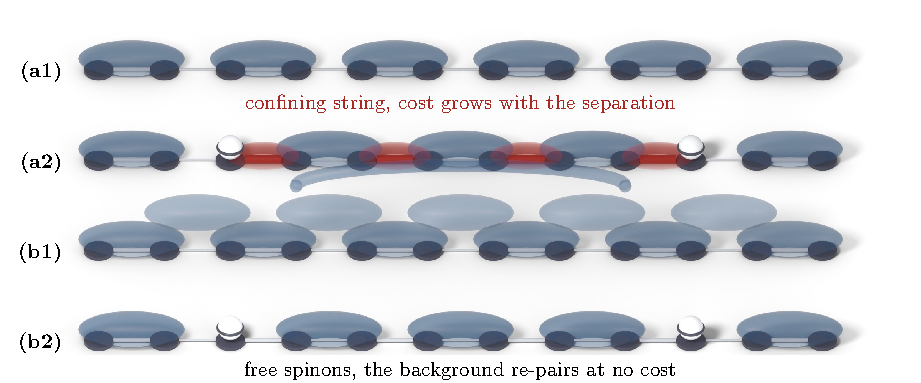
\includegraphics{figures/pdf/s08f03_vbs_rvb.pdf}
\end{aqmfigure}
